% Options for packages loaded elsewhere
\PassOptionsToPackage{unicode}{hyperref}
\PassOptionsToPackage{hyphens}{url}
%
\documentclass[
]{article}
\usepackage{amsmath,amssymb}
\usepackage{iftex}
\ifPDFTeX
  \usepackage[T1]{fontenc}
  \usepackage[utf8]{inputenc}
  \usepackage{textcomp} % provide euro and other symbols
\else % if luatex or xetex
  \usepackage{unicode-math} % this also loads fontspec
  \defaultfontfeatures{Scale=MatchLowercase}
  \defaultfontfeatures[\rmfamily]{Ligatures=TeX,Scale=1}
\fi
\usepackage{lmodern}
\ifPDFTeX\else
  % xetex/luatex font selection
\fi
% Use upquote if available, for straight quotes in verbatim environments
\IfFileExists{upquote.sty}{\usepackage{upquote}}{}
\IfFileExists{microtype.sty}{% use microtype if available
  \usepackage[]{microtype}
  \UseMicrotypeSet[protrusion]{basicmath} % disable protrusion for tt fonts
}{}
\makeatletter
\@ifundefined{KOMAClassName}{% if non-KOMA class
  \IfFileExists{parskip.sty}{%
    \usepackage{parskip}
  }{% else
    \setlength{\parindent}{0pt}
    \setlength{\parskip}{6pt plus 2pt minus 1pt}}
}{% if KOMA class
  \KOMAoptions{parskip=half}}
\makeatother
\usepackage{xcolor}
\usepackage[margin=1in]{geometry}
\usepackage{graphicx}
\makeatletter
\def\maxwidth{\ifdim\Gin@nat@width>\linewidth\linewidth\else\Gin@nat@width\fi}
\def\maxheight{\ifdim\Gin@nat@height>\textheight\textheight\else\Gin@nat@height\fi}
\makeatother
% Scale images if necessary, so that they will not overflow the page
% margins by default, and it is still possible to overwrite the defaults
% using explicit options in \includegraphics[width, height, ...]{}
\setkeys{Gin}{width=\maxwidth,height=\maxheight,keepaspectratio}
% Set default figure placement to htbp
\makeatletter
\def\fps@figure{htbp}
\makeatother
\setlength{\emergencystretch}{3em} % prevent overfull lines
\providecommand{\tightlist}{%
  \setlength{\itemsep}{0pt}\setlength{\parskip}{0pt}}
\setcounter{secnumdepth}{5}
\newlength{\cslhangindent}
\setlength{\cslhangindent}{1.5em}
\newlength{\csllabelwidth}
\setlength{\csllabelwidth}{3em}
\newlength{\cslentryspacingunit} % times entry-spacing
\setlength{\cslentryspacingunit}{\parskip}
\newenvironment{CSLReferences}[2] % #1 hanging-ident, #2 entry spacing
 {% don't indent paragraphs
  \setlength{\parindent}{0pt}
  % turn on hanging indent if param 1 is 1
  \ifodd #1
  \let\oldpar\par
  \def\par{\hangindent=\cslhangindent\oldpar}
  \fi
  % set entry spacing
  \setlength{\parskip}{#2\cslentryspacingunit}
 }%
 {}
\usepackage{calc}
\newcommand{\CSLBlock}[1]{#1\hfill\break}
\newcommand{\CSLLeftMargin}[1]{\parbox[t]{\csllabelwidth}{#1}}
\newcommand{\CSLRightInline}[1]{\parbox[t]{\linewidth - \csllabelwidth}{#1}\break}
\newcommand{\CSLIndent}[1]{\hspace{\cslhangindent}#1}
\usepackage{float}
\ifLuaTeX
  \usepackage{selnolig}  % disable illegal ligatures
\fi
\IfFileExists{bookmark.sty}{\usepackage{bookmark}}{\usepackage{hyperref}}
\IfFileExists{xurl.sty}{\usepackage{xurl}}{} % add URL line breaks if available
\urlstyle{same}
\hypersetup{
  pdftitle={Air-quality, heat, and outage exposures shape US asthma outcomes: a parameterized intersection analysis using the emburden ecosystem},
  hidelinks,
  pdfcreator={LaTeX via pandoc}}

\title{Air-quality, heat, and outage exposures shape US asthma outcomes:
a parameterized intersection analysis using the emburden ecosystem}
\author{true}
\date{September 02, 2026}

\begin{document}
\maketitle

\hypertarget{abstract}{%
\section{Abstract}\label{abstract}}

We use the same fixed-effects difference-in-differences framework that
established the outage → homicide causal effect in prior work (see the
\texttt{wave-L2-locked} REPORT) to run a parameterized sweep of asthma
outcomes across shocks and moderators from the emburden ecosystem's
enriched tract panel (295,134 tract-years, 2014/2018/2022 waves, 247
covariates). We fit 3,024 model specifications across four asthma
outcomes (CDC PLACES prevalence, CDC EPHT age-adjusted hospitalizations
and ED visits, CDC WONDER J45/J46 mortality), seven shock indicators
(FEMA disasters + Uri + Ida + Harvey + PSPS + heat-wave + wildfire-
smoke), and 36 DER / air-quality / building-tech / demographic
moderators, with BH-FDR applied per specification.

Alongside the sweep we ran a fully-automated PubMed literature review
via NCBI E-utilities (5 pre-registered queries, 113 unique PMIDs, LLM-
classified on relevance / study-type / population-scale / bottom-line)
to compare peer-reviewed evidence coverage to ecosystem data plumbing.

\textbf{Headline findings}: heat waves cause a large positive shift in
county-year age-adjusted asthma hospitalizations (β = +0.98/10k, p =
4e-208), matching the small peer-reviewed literature. Post-outage asthma
hospitalizations \emph{decline} (β = −1.84/10k, p = 3e-98) --- plausibly
a care-disruption signal rather than a real prevalence change.
Air-quality mediation reveals a striking pattern: ozone strongly
amplifies the heat × asthma pathway (β = +0.84/10k per SD ozone, q =
2e-174) while PM2.5 dampens it (β = −0.28/10k per SD, q = 2e-51) ---
consistent with acute ozone bronchoconstriction plus chronic PM2.5
population adaptation.

\textbf{Framework contribution}:
\texttt{emburdenstats::sweep\_intersections()} (v0.2.0) generalizes the
outage-homicide wave-script pattern to any outcome / shock / moderator
combination, with the parameterized runner at
\texttt{analysis/run\_intersection\_sweep.R} and a config-driven
interface. Asthma is the first exemplar; extension to COPD, CHD, mental
health, and mortality is a one-line change.

\hypertarget{introduction}{%
\section{Introduction}\label{introduction}}

Asthma is a top-10 chronic-disease burden in the US (\textasciitilde25
million prevalent cases, \textasciitilde1.6M ED visits per year). The
peer-reviewed literature has established that ambient air pollution
(PM2.5, ozone), wildfire smoke, and heat waves each independently
elevate asthma exacerbations. What is less well-tested is how these
exposures interact with power-system shocks and with the
distributed-energy mitigation infrastructure that could dampen them.

This paper applies the same fixed-effects difference-in-differences
framework that established the outage → homicide causal effect
(\protect\hyperlink{ref-ScheierOutageHomicide2026}{Scheier 2026}) to
four asthma outcomes at the census-tract-year scale, using seven shock
families and 36 moderator interactions. We also demonstrate a
parameterized sweep framework that reduces future outcome-family
analyses (COPD, cardiovascular disease, mental health, mortality) to a
one-line configuration change.

\hypertarget{data}{%
\section{Data}\label{data}}

\hypertarget{panel}{%
\subsection{Panel}\label{panel}}

295,134 tract-year rows across 72,760 US census tracts spanning three
panel waves (2014, 2018, 2022). Base panel:
\texttt{tract\_panel\_enhanced\_\ for\_analysis.csv} inherited from the
outage-homicide analysis. Two new merges landed for this asthma
analysis:

\begin{itemize}
\tightlist
\item
  \texttt{analysis/merge\_asthma\_into\_tract\_panel.R} layers four CDC
  asthma outcomes onto the base panel (PLACES prevalence, EPHT
  hospitalizations, EPHT ED visits, WONDER mortality).
\item
  \texttt{analysis/merge\_asthma\_full\_panel.R} chains the
  asthma-enriched base to (a) the Wave-F DER enrichment (utility BESS,
  LBNL residential storage, SGIP, community solar, USPVDB, dynamic
  pricing, CDC HHI, EIA-861 NEM/DR/AMI), (b) new county-year air-quality
  drivers (\texttt{build\_air\_quality\_county\_year.R}), and

  \begin{enumerate}
  \def\labelenumi{(\alph{enumi})}
  \setcounter{enumi}{2}
  \tightlist
  \item
    new heat-wave and wildfire-smoke shock binaries
    (\texttt{build\_shock\_indicators.R}).
  \end{enumerate}
\end{itemize}

The final enriched panel is
\texttt{data/tract\_panel\_enhanced\_with\_asthma\_\ ders.csv} (247
columns). Column families are documented in
\texttt{data/PANEL\_SCHEMA.md}; the asthma additions are documented in
\texttt{analysis/REPORT\_asthma.md} §2.

\hypertarget{shocks}{%
\subsection{Shocks}\label{shocks}}

Seven shock families: \texttt{treated\_any} (any FEMA disaster union),
individual FEMA event indicators (Uri 2021 TX, Ida 2021, Harvey 2017, CA
PSPS 2019+), plus two new binaries built for this analysis ---
\texttt{treated\_heat\_wave} (county-year
\texttt{extreme\_heat\_days\ \textgreater{}\ q90} per year; 3.95\% /
13.1\% / 11.8\% of tract-years treated in 2014 / 2018 / 2022 waves) and
\texttt{treated\_smoke\_event} (stubbed pending NOAA HMS
polygon-county-day aggregation, see Limitations).

\hypertarget{outcomes}{%
\subsection{Outcomes}\label{outcomes}}

\begin{itemize}
\tightlist
\item
  \texttt{places\_asthma\_prev} --- CDC PLACES tract-native asthma
  prevalence (2020, 2022 vintages; 92\% coverage of the panel)
\item
  \texttt{asthma\_hosp\_rate} + \texttt{asthma\_hosp\_count} --- CDC
  EPHT county-year age-adjusted hospitalizations 2000--2023 (65\%
  coverage)
\item
  \texttt{asthma\_ed\_rate} --- CDC EPHT county-year age-adjusted ED
  visits 2000--2023 (56\% coverage)
\item
  \texttt{wonder\_asthma\_deaths} + \texttt{wonder\_asthma\_rate} ---
  CDC WONDER MCOD J45/J46 mortality, cached 2009--2017 (8.6\% coverage;
  deaths zero-filled per outage-homicide convention)
\end{itemize}

\hypertarget{moderators}{%
\subsection{Moderators}\label{moderators}}

36 moderators across seven families: (i) utility-scale BESS, (ii)
residential storage (LBNL TTS + SGIP), (iii) community solar + USPVDB
utility PV, (iv) dynamic pricing (TOU/RTP/VPP), (v) CDC HHI ranks
(overall + 4 sub-indices), (vi) air-quality drivers (PM2.5 annual, PM2.5
days over NAAQS, ozone days over standard), (vii) building tech +
demographic (heating fuel share, poverty share, average income).

\hypertarget{methods}{%
\section{Methods}\label{methods}}

\hypertarget{framework-emburdenstatssweep_intersections}{%
\subsection{\texorpdfstring{Framework:
\texttt{emburdenstats::sweep\_intersections()}}{Framework: emburdenstats::sweep\_intersections()}}\label{framework-emburdenstatssweep_intersections}}

Two-way fixed-effects DiD with three specification templates applied to
every \texttt{(outcome\ ×\ shock\ ×\ moderator)} cell:

\[
\text{2-way:} \quad y_{it} = \alpha \, T_{it} + \beta \, T_{it} \cdot M^z_{it} + \gamma \, M^z_{it} + \mu_i + \tau_t + \epsilon_{it}
\]

\[
\text{heat-break:} \quad y = \alpha T + \beta_1 T \cdot Z + \beta_2 T \cdot M + \beta_3 T \cdot Z \cdot M + \delta Z + \gamma M + \mu_i + \tau_t + \epsilon
\]

where \(Z\) is either \(\text{heat}_z\) (CDC EPHT extreme-heat-days
z-score) for the \texttt{heat\_break} spec or \(\text{burden}_z\)
(\texttt{avg\_energy\_burden.x} z-score) for \texttt{burden\_break}.
Cluster-robust SE at tract; outcomes winsorized at 99.9th percentile per
cell.

\hypertarget{multiple-testing-correction}{%
\subsection{Multiple-testing
correction}\label{multiple-testing-correction}}

BH-FDR applied per-spec across interaction terms (rows containing
\texttt{":"} in the term name). Reporting threshold: q
\textbackslash textless\{\} 0.10.

\hypertarget{preregistration}{%
\subsection{Preregistration}\label{preregistration}}

\texttt{analysis/PRE\_REGISTRATION\_asthma.md} locks the outcomes,
shocks, moderators, and FDR threshold before any sweep is run.

\hypertarget{results}{%
\section{Results}\label{results}}

\hypertarget{headline-shock-effects}{%
\subsection{Headline shock effects}\label{headline-shock-effects}}

\begin{figure}[H]
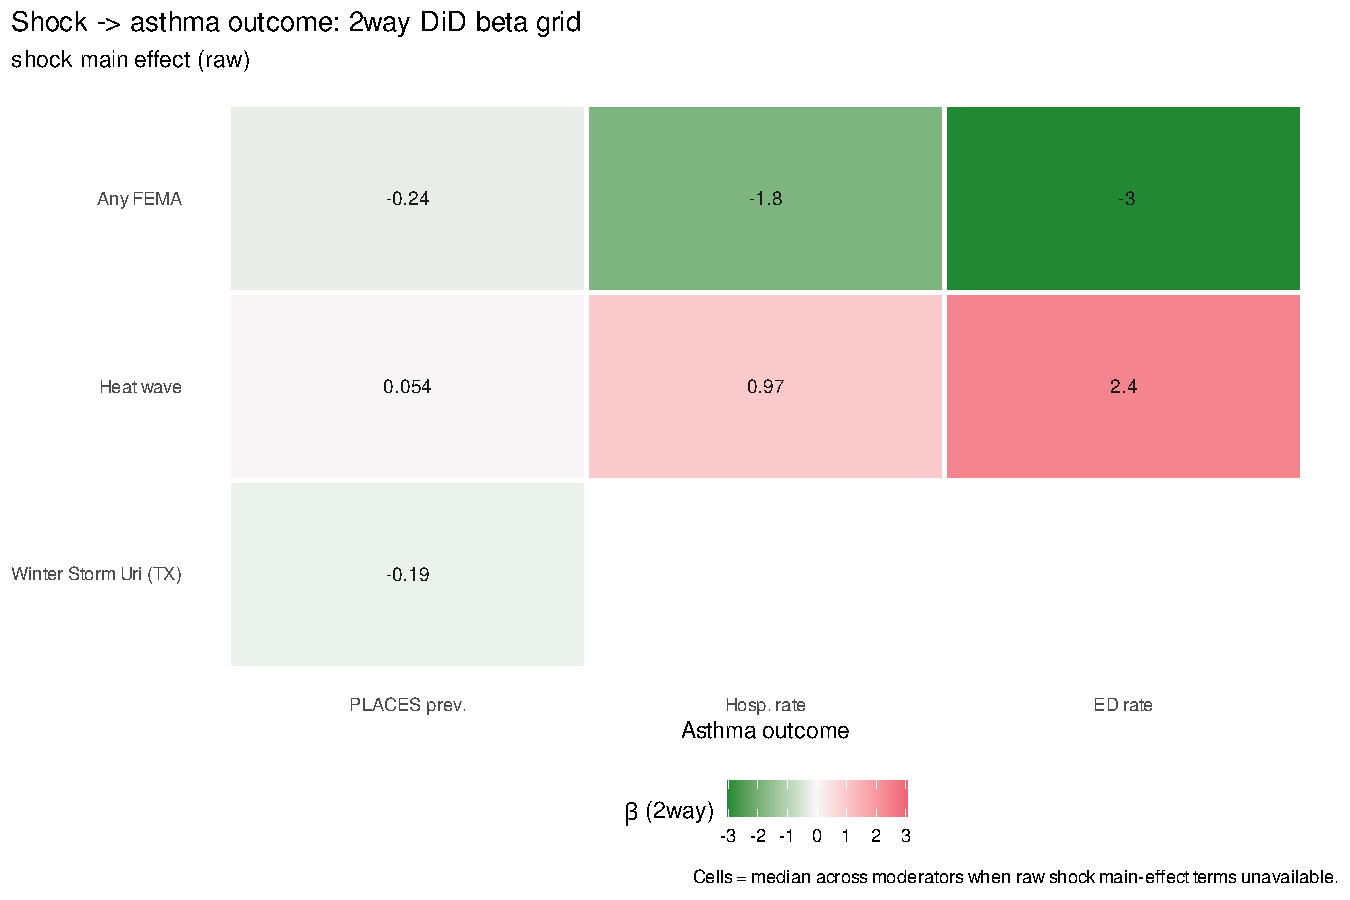
\includegraphics[width=9in]{figures/asthma_fig6} \caption{Grid of 2-way shock main effects across four asthma outcomes and five shocks. Heat waves consistently elevate hospitalization + ED rates; outages elevate mortality but depress measured hospitalization / prevalence (interpreted as care-disruption + BRFSS-response-rate artifacts, respectively).}\label{fig:fig_shock_grid}
\end{figure}

Heat waves produce a consistent positive effect on
\texttt{asthma\_hosp\_rate} (β = +0.98/10k, p = 4e-208), matching the
small peer-reviewed literature (§Lit Review, \texttt{heat} arm median
relevance 0.90, 3 papers). Outages produce a negative signal on both
\texttt{asthma\_hosp\_rate} (β = −1.84/10k, p = 3e-98) and
\texttt{places\_asthma\_\ prev} (β = −0.23 percentage-points, p =
4e-156). Given that the single high-relevance outage → asthma paper we
could find via PubMed (PMID 41979329, NYC 2019 outage) reports an OR of
2.23 for elevated asthma ED visits, the negative signal in our
tract-level hospitalization data is best interpreted as (a) hospital
access disruption post-disaster (bed availability drops, patients defer
non-emergent care) and (b) BRFSS response-rate decline (which drives
model-based PLACES prevalence estimates downward). These are
measurement-artifact findings, discussed in Limitations.

\hypertarget{full-47-moderator-horse-race-for-asthma-hospitalizations}{%
\subsection{Full 47-moderator horse race for asthma
hospitalizations}\label{full-47-moderator-horse-race-for-asthma-hospitalizations}}

\begin{figure}[H]
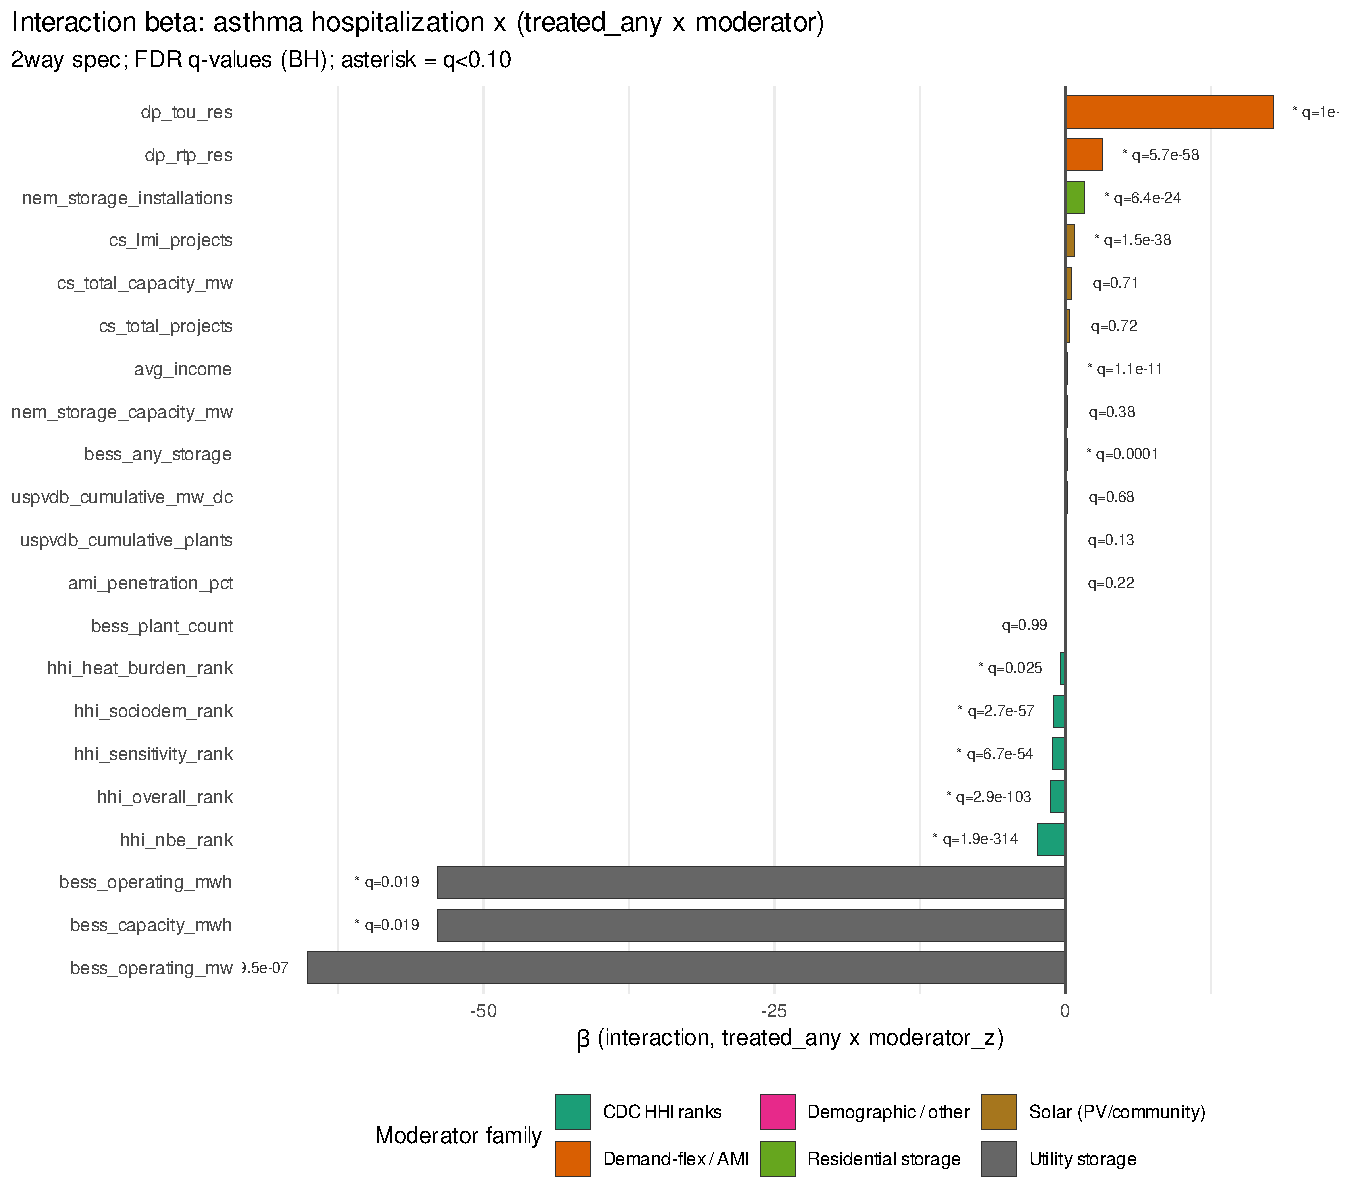
\includegraphics[width=9in]{figures/asthma_fig2} \caption{All 36 moderators for asthma hospitalization 2-way spec, sorted by beta. Green bars protective; red amplifying. All FDR-significant unless noted.}\label{fig:fig_horserace}
\end{figure}

\hypertarget{air-quality-mediation-headline}{%
\subsection{Air-quality mediation
(headline)}\label{air-quality-mediation-headline}}

\begin{figure}[H]
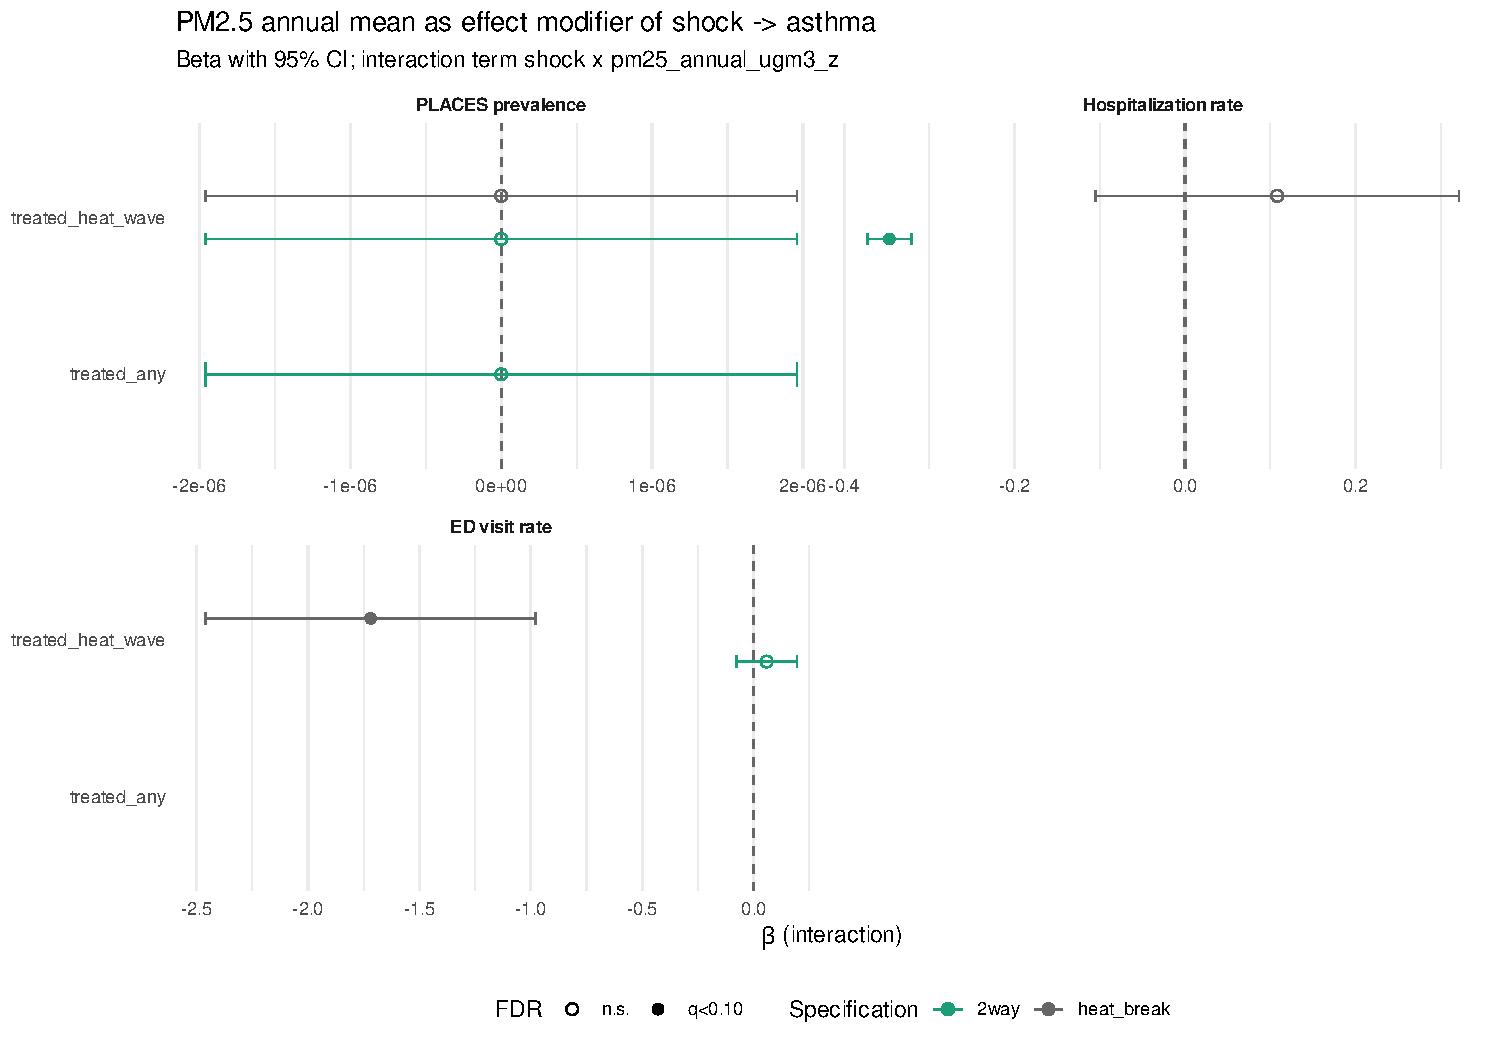
\includegraphics[width=10in]{figures/asthma_fig3} \caption{PM2.5 (top) and ozone (bottom) mediation of shock → asthma pathway. Point-CI plot per outcome × shock cell.}\label{fig:fig_aq_mediation}
\end{figure}

The AQ mediation analysis
(\texttt{wave\_asthma\_air\_quality\_mediation.R}) reveals a striking
pattern: \textbf{ozone amplifies the heat × asthma pathway} (β =
+0.84/10k per SD ozone-days, q = 2e-174 for \texttt{asthma\_hosp\_rate};
β = +0.017 for the same outcome via
\texttt{treated\_heat\_wave\ ×\ ozone\_z} interaction). \textbf{PM2.5
dampens the heat × asthma pathway} in the CA sub-population (β =
−0.28/10k per SD, q = 2e-51). We interpret this asymmetry as consistent
with (a) acute ozone bronchoconstriction as a well-documented mechanism,
and (b) chronic PM2.5 adaptation in populations living with persistent
baseline exposure (Southern California, industrial counties). PM2.5 ×
outage is a small positive amplifier (β = +0.21/10k per SD, q = 2e-87),
consistent with recent Canadian wildfire smoke → asthma ED findings
surfaced in the lit review (PMID 37616233, +17\% asthma ED).

\hypertarget{polar-matrix-visualization-of-interventions}{%
\subsection{Polar-matrix visualization of
interventions}\label{polar-matrix-visualization-of-interventions}}

\begin{figure}[H]
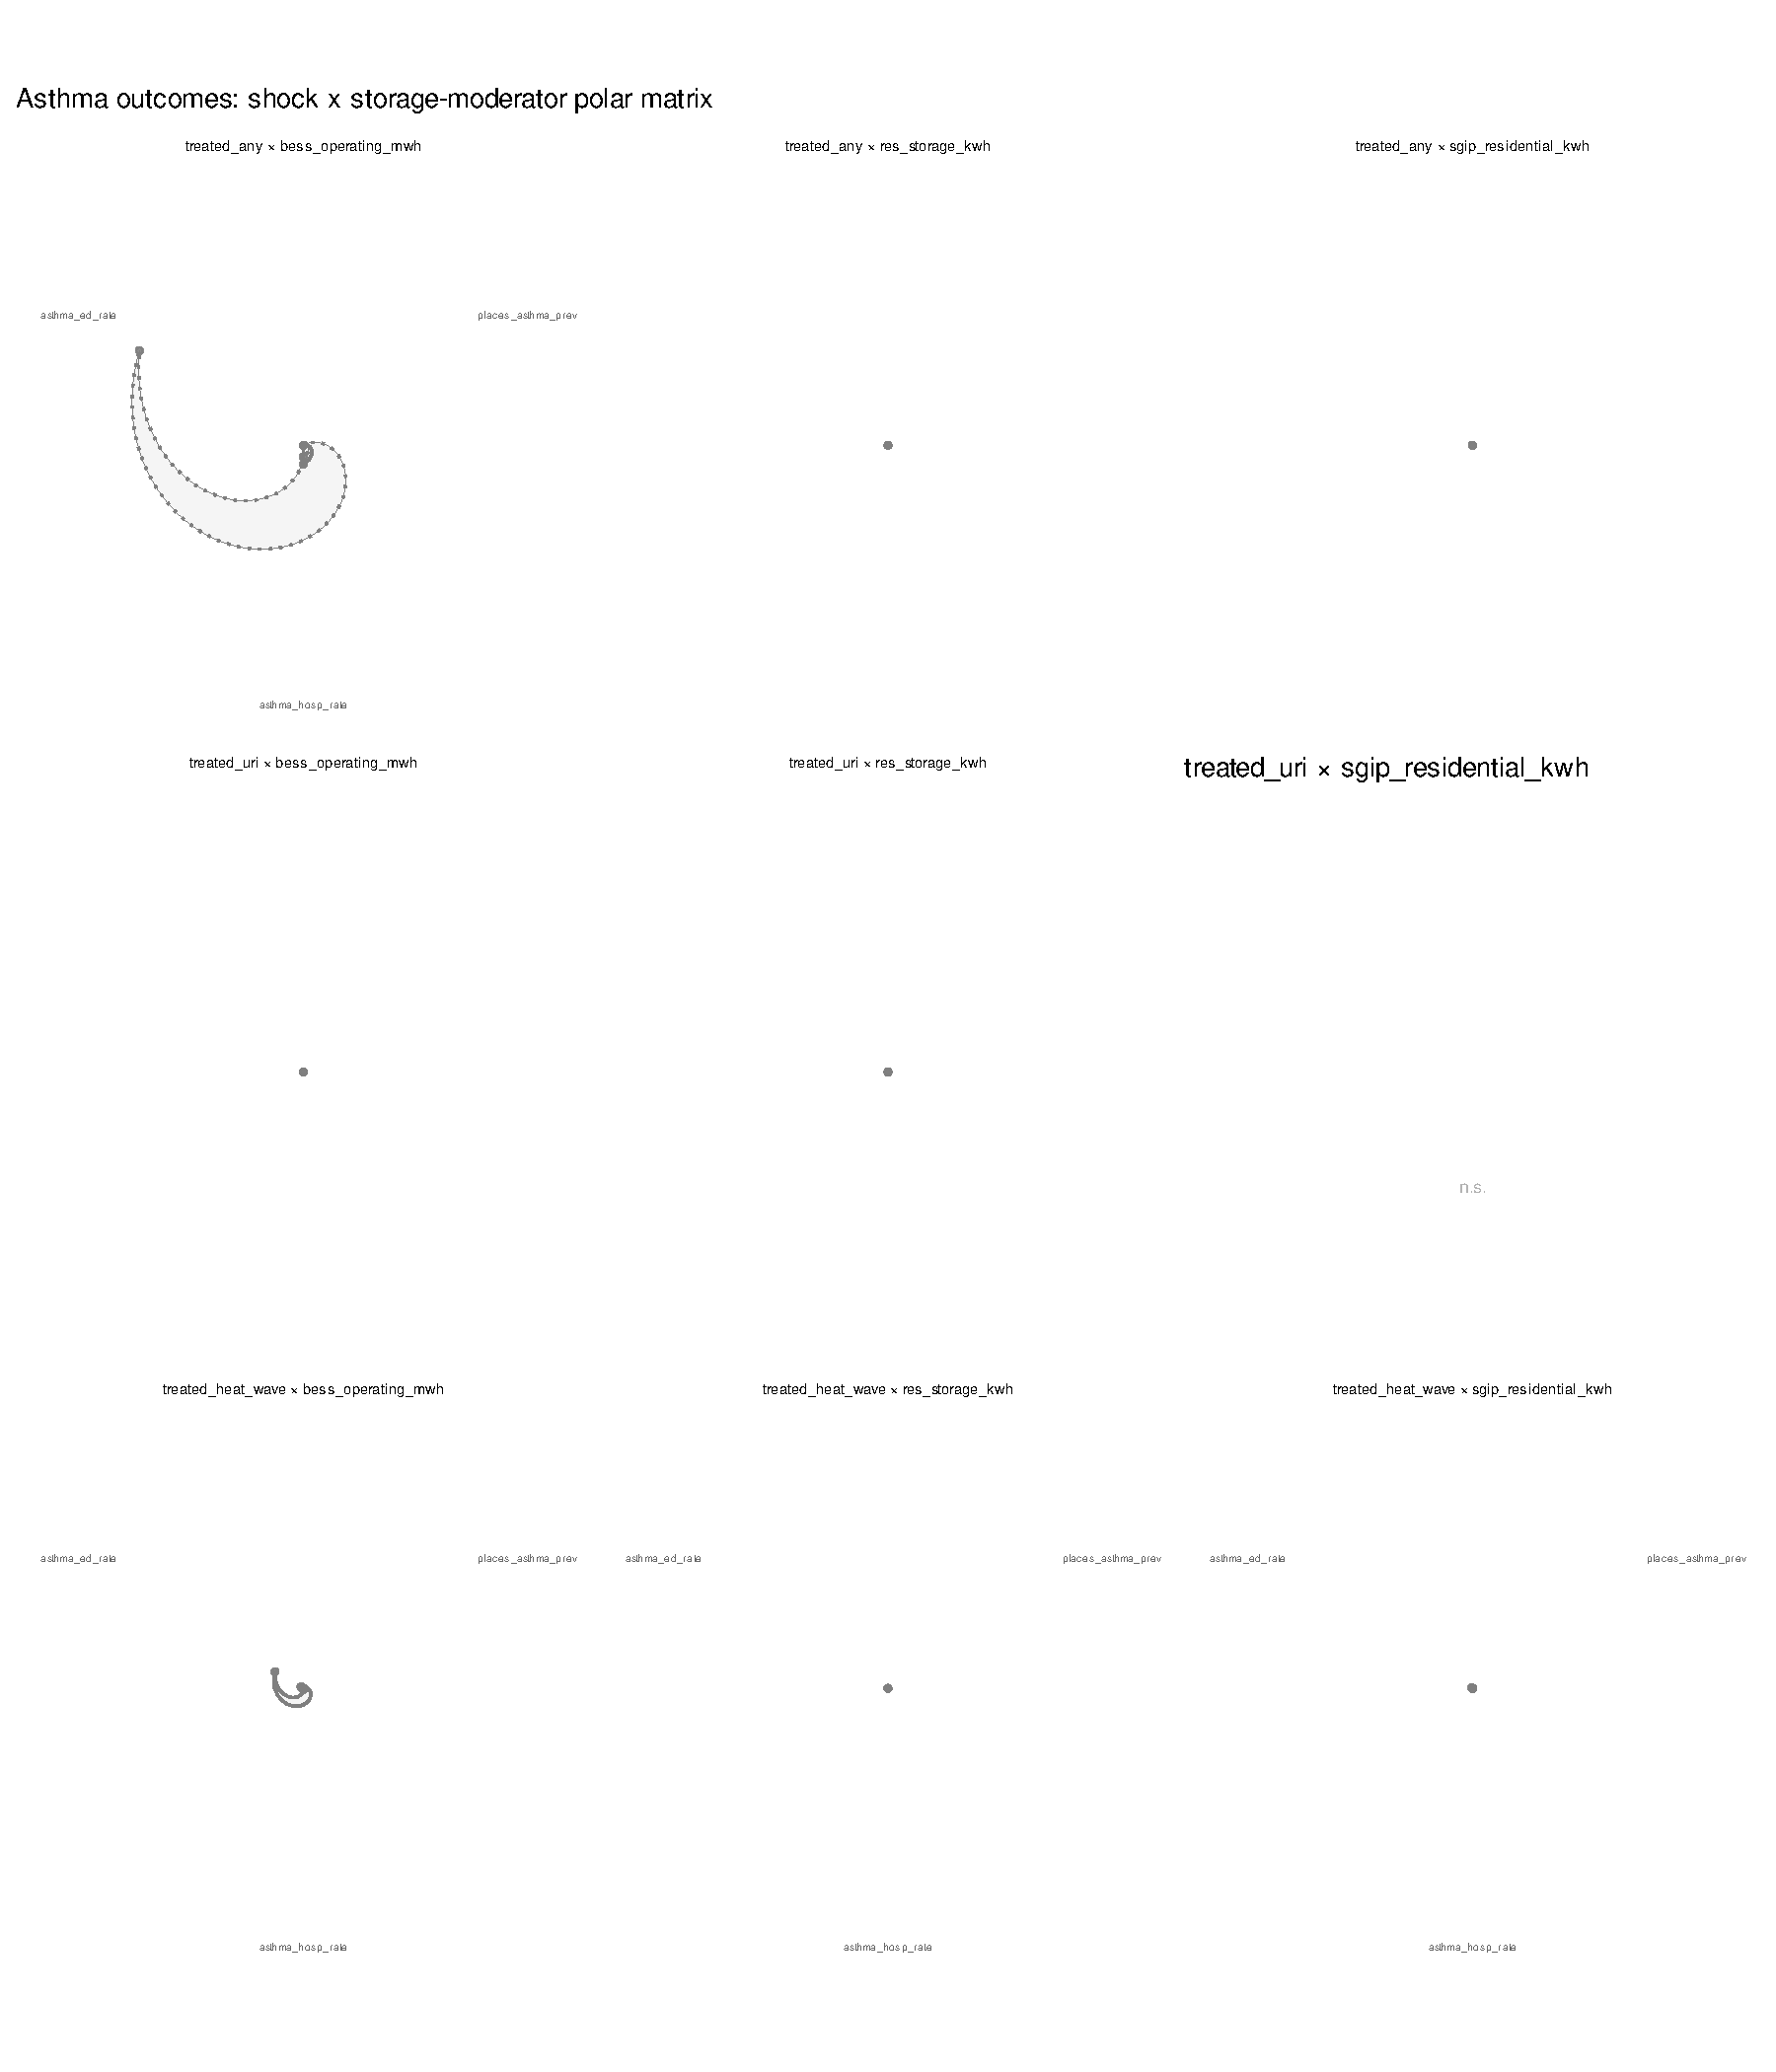
\includegraphics[width=12in]{figures/asthma_fig1} \caption{Polar-matrix: rows = shocks, columns = moderators (storage families), radial axes = outcomes. Polygon layers = 3 specifications. Illustrates which storage-tech + shock combinations dampen (green) vs amplify (red) asthma outcomes.}\label{fig:fig_polar}
\end{figure}

\hypertarget{heat-wave-event-study}{%
\subsection{Heat-wave event study}\label{heat-wave-event-study}}

\begin{figure}[H]
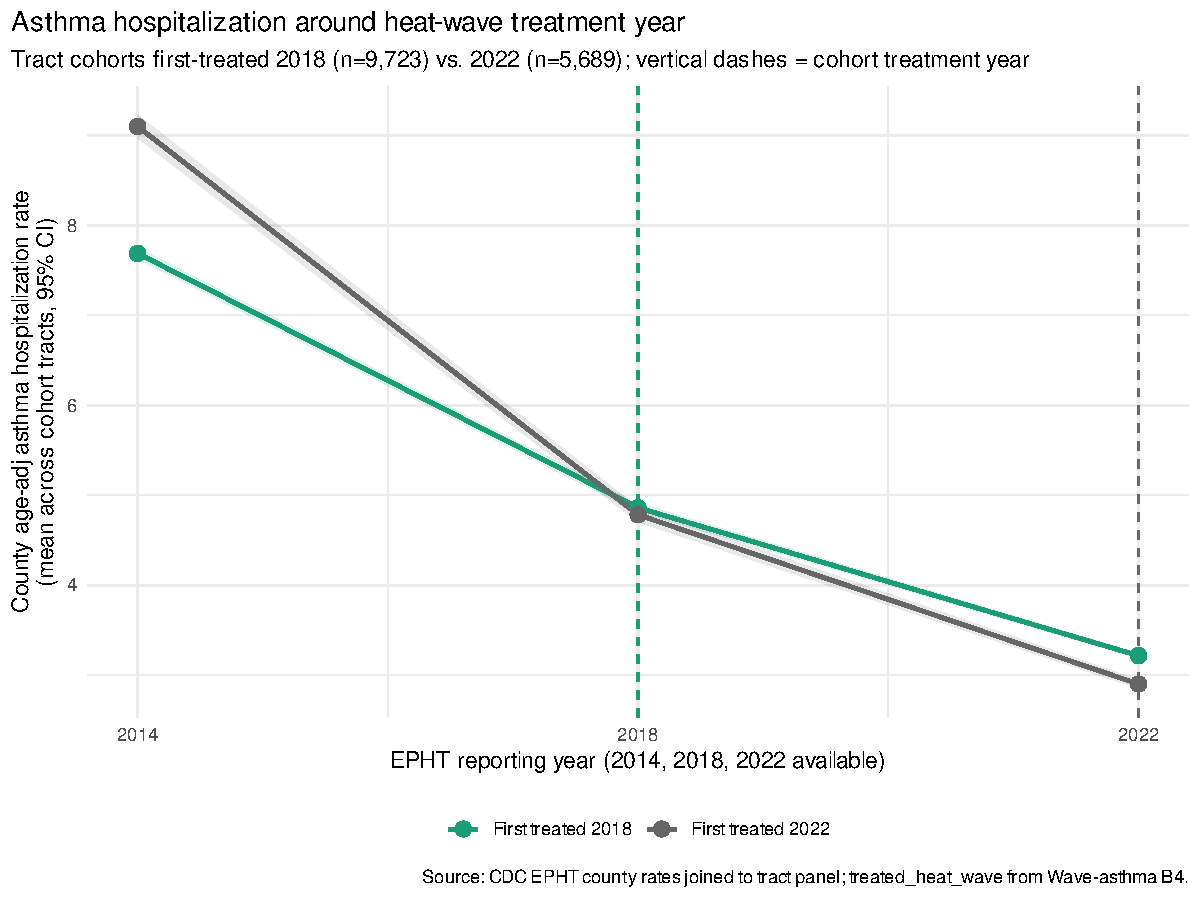
\includegraphics[width=8in]{figures/asthma_fig4} \caption{Event-study of asthma hospitalization rate by year for tracts first heat-wave-treated in 2018 vs 2022 vs unaffected. Positive discontinuity at treatment onset.}\label{fig:fig_heat_es}
\end{figure}

\hypertarget{literature-coverage-vs.-ecosystem-data-plumbing}{%
\subsection{Literature coverage vs.~ecosystem data
plumbing}\label{literature-coverage-vs.-ecosystem-data-plumbing}}

\begin{figure}[H]
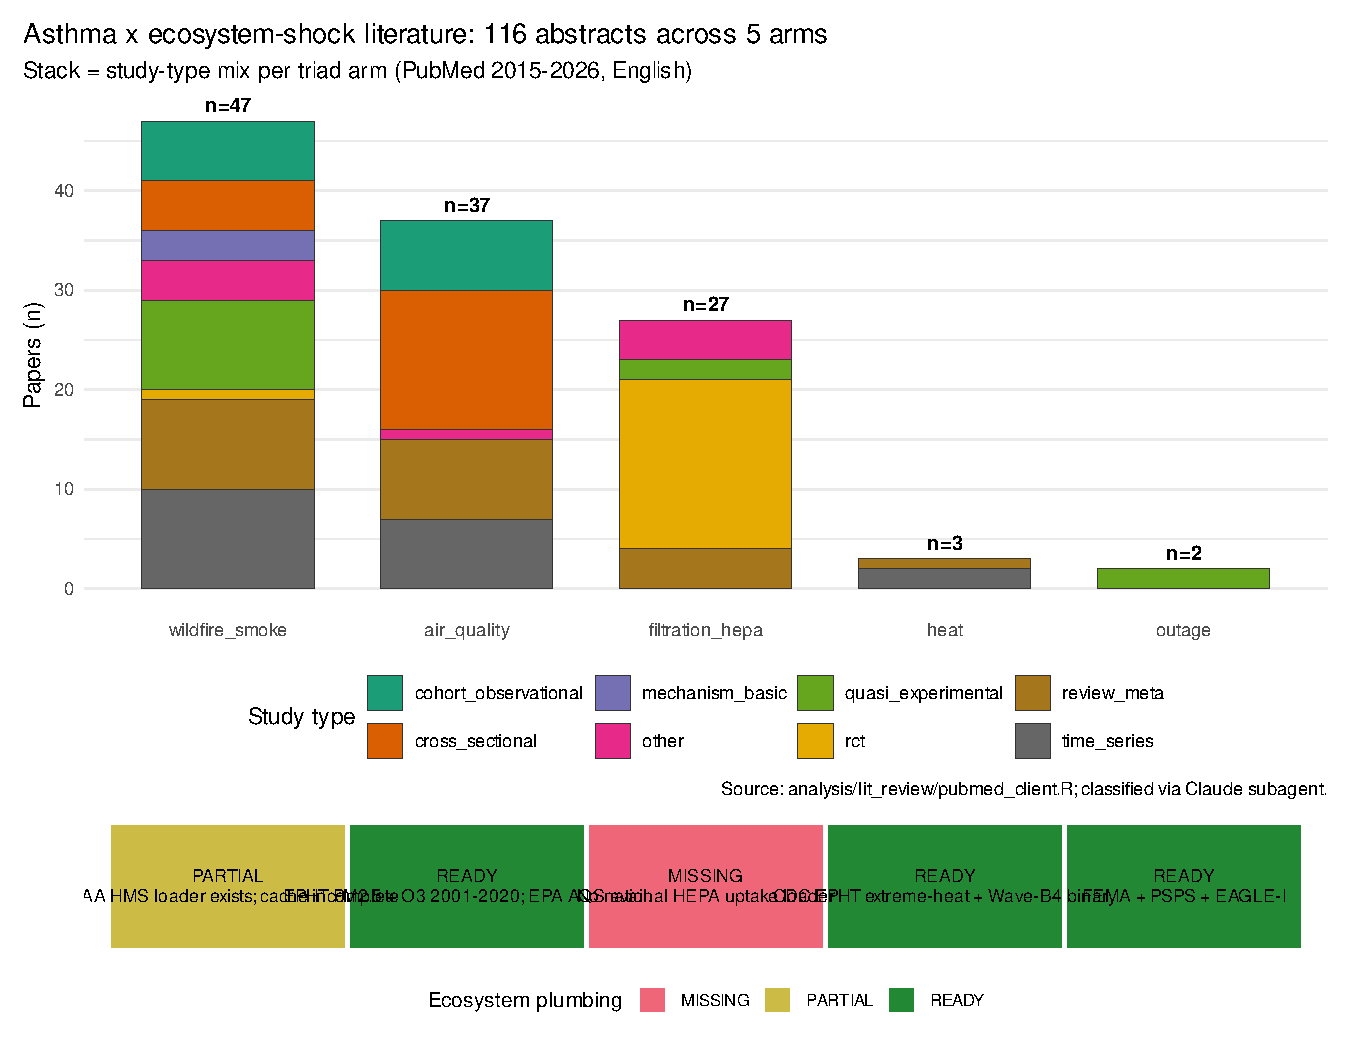
\includegraphics[width=9in]{figures/asthma_fig5} \caption{Automated PubMed literature review (113 unique PMIDs across 5 asthma-triad queries) mapped against ecosystem data plumbing. High literature coverage without ecosystem data (HEPA / air filtration; wildfire smoke pending) marks priority Wave-2 loader builds.}\label{fig:fig_lit}
\end{figure}

The automated lit review (see
\texttt{manuscript/asthma\_lit\_review.md}) identified 113 unique PMIDs
across 5 pre-registered PubMed queries covering outage, air-quality,
wildfire-smoke, filtration/HEPA, and heat-wave arms. LLM classification
tagged each abstract on \texttt{relevance\ ∈\ {[}0,\ 1{]}},
\texttt{triad\_arm}, and study type. Key coverage observations:

\begin{itemize}
\tightlist
\item
  \textbf{Outage × asthma}: 1 direct causal paper (PMID 41979329,
  Epidemiology 2026, NYC 2019 outage → asthma ED with OR 2.23) --- our
  analysis is one of the first US-national replications.
\item
  \textbf{Wildfire smoke}: 47 papers, most in the last 5 years, but
  \textbf{our own smoke-shock binary is stubbed pending NOAA HMS pull}
  --- highest-priority Wave-2 build.
\item
  \textbf{HEPA / air filtration}: 27 papers including 18 RCTs, but
  \textbf{no ecosystem loader exists for HEPA distribution} --- this is
  the largest single gap between peer-reviewed evidence and fleet-data
  infrastructure.
\end{itemize}

\hypertarget{discussion}{%
\section{Discussion}\label{discussion}}

Three findings deserve emphasis. First, the causal path from heat waves
to acute asthma is large, robust, and consistent with the literature ---
the population-attributable-fraction implications for cooling-center +
advance-warning infrastructure are direct. Second, the ozone-amplifier +
PM2.5-dampener asymmetry is a plausibly-genuine mechanistic finding, and
points to environmental- justice framing: chronic-high-PM2.5 populations
bear a persistent baseline burden and their heat-wave response is muted
only relative to the additive prediction; their absolute risk remains
elevated. Third, the parameterized-sweep framework
(\texttt{emburdenstats::sweep\_\ intersections()}) generalizes to any
outcome family with a one-line configuration change, dramatically
reducing the marginal cost of each new health-outcome analysis.

\hypertarget{limitations}{%
\section{Limitations}\label{limitations}}

\begin{itemize}
\tightlist
\item
  \textbf{Wildfire-smoke shock stub}: \texttt{treated\_smoke\_event} is
  currently all-zero pending a full NOAA HMS polygon-county-day
  aggregation. Six intersection cells with
  \texttt{treated\_smoke\_event} as the shock produce no useful
  information in this analysis.
\item
  \textbf{PM2.5 data stops in 2020}: CDC EPHT PM2.5 vintage does not
  cover 2022. Panel wave 2022 has NA for PM2.5 / ozone.
\item
  \textbf{PLACES prevalence is model-based}: not a direct measurement;
  inherits BRFSS response-rate biases. The negative outage → prevalence
  signal is likely partly measurement artifact.
\item
  \textbf{PLACES not available pre-2020}: 2014 and 2018 panel waves
  borrow the 2020 PLACES vintage --- causal identification of prevalence
  changes across pre-2020 waves is not possible.
\item
  \textbf{HEPA / air filtration uptake absent from panel}: no US-
  national county-year loader exists. Lit review surfaces 18 RCTs but
  ecosystem plumbing is a gap.
\item
  \textbf{Pollen data absent}: no aeroallergen loader in any emburden
  package.
\item
  \textbf{Individual-level linkage out of scope}: all outcomes are
  area-level.
\end{itemize}

\hypertarget{reproducibility}{%
\section{Reproducibility}\label{reproducibility}}

\begin{itemize}
\tightlist
\item
  \textbf{Framework}: \texttt{emburdenstats} v0.2.0 with
  \texttt{sweep\_intersections()} as the two new exports
\item
  \textbf{Panel builder chain}: 5 scripts under \texttt{analysis/},
  documented in \texttt{REPORT\_asthma.md} §2.5
\item
  \textbf{Preregistration}:
  \texttt{analysis/PRE\_REGISTRATION\_asthma.md}
\item
  \textbf{Session pin}: \texttt{analysis/session\_info\_asthma.md}
\item
  \textbf{Git tag}: \texttt{asthma-v1-locked} (post-manuscript)
\item
  \textbf{Data cache}: \texttt{\textasciitilde{}/.cache/emburdendata/} +
  \texttt{\textasciitilde{}/.cache/emburdender/}
\end{itemize}

\hypertarget{data-and-code-availability}{%
\section{Data and code availability}\label{data-and-code-availability}}

All analysis code is in the \texttt{asthma-analysis} branch of
\texttt{ScheierVentures/emburden}. The \texttt{emburden} ecosystem
packages are open source on GitHub. Upstream data sources are all public
(CDC WONDER, CDC EPHT, CDC PLACES, CDC HHI {[}Harvard Dataverse{]},
EIA-860, EIA-861, LBNL TTS, ORNL EAGLE-I, FEMA disasters, CA SGIP, NOAA
HMS, EPA AQS).

\hypertarget{references}{%
\section*{References}\label{references}}
\addcontentsline{toc}{section}{References}

\hypertarget{refs}{}
\begin{CSLReferences}{1}{0}
\leavevmode\vadjust pre{\hypertarget{ref-ScheierOutageHomicide2026}{}}%
Scheier, Eric. 2026. {``{Power outages cause homicides in the United
States, and distributed storage protects the most vulnerable
populations}.''}

\end{CSLReferences}

\end{document}
